\documentclass{report}
\usepackage{graphicx}

\begin{document}
\flushleft


\includegraphics[scale=0.08]{figure/logo-aka.jpg}
\section*{Aikikai Australia Class Attendance System}

Aikikai Australia has set up a new web based class attendance system.
This new system will allows us to maintain more accurate attendance records,
reduce the administration burden to maintain these records,
and help determine student-to-student contacts in the case of COVID-19 infection.
The system is currently being trialed by a few dojos in NSW. The trial will
be expanded once we are happy that the system is sufficiently stable and usable.

\smallskip
The new system is based on QR (Quick Response) codes, similar to those used
at other organisations and businesses to track attendance to their venues.

\medskip
We use a two step workflow:

\subsection*{1. Student Registration}
\begin{center}
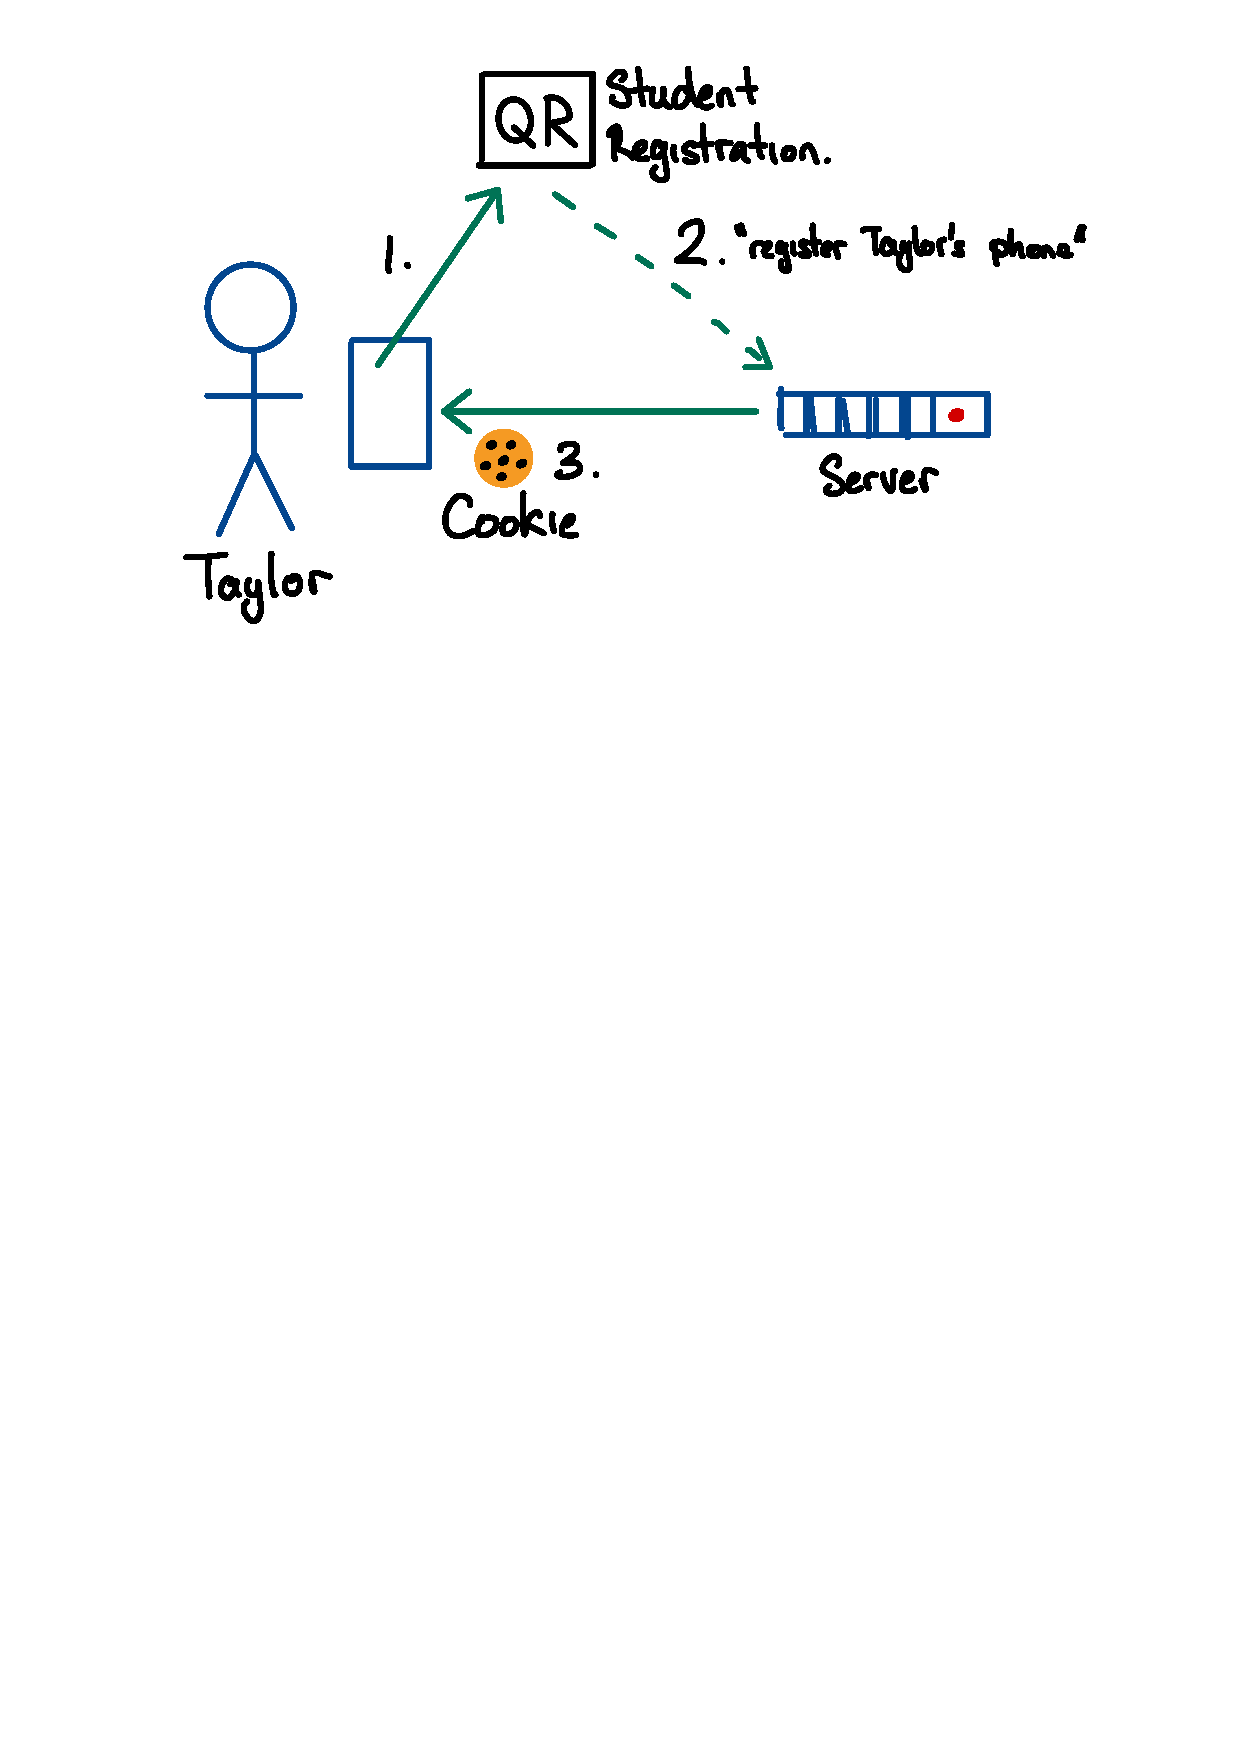
\includegraphics[scale=0.4]{figure/fig-student-registration.pdf}
\end{center}

\begin{enumerate}
\item The student (here, Taylor) uses their phone to scan their personal
      registration QR code.

\item The QR code redirects the student's phone to the attendance server,
      instructing the server to register the phone as belonging to this student.

\item The server provides a \emph{cookie} (a special code) that includes
      the Aikikai identification number of that student. The phone stores
      this cookie, and will give a copy back to the server if later requested.
\end{enumerate}

Each student needs to perform this process to register with the system.
They may need to register again if they change phones, or if they instruct the
web browser on their phone to clear the cookies it is holding.



\subsection*{Frequently Asked Questions}
\begin{enumerate}
\item Q. What if I don't have a phone, or forget to bring it?
      A. The class instructor can add your name to the attendance list
         directly on the server, via a separate web page.

\item Q. Who has access to the attendance records?
      A. Instructors and adminstrators that are part of Aikikai Australia.
         The physical computer that the site runs on is hosted by a professional hosting
         company (Linode), and is located in Sydney, Australia. The hosting company
         has access to the physical machine, which is common to other professionally
         hosted sites. The server does not run any other services besides the
         attendance system.

\item Q. Does clearing cookies from my phone affect my attendance records on the server?
      A. No. The cookie only contains your encoded Aikikai identification number.
         The cookie is used by the server to determine which student owns the phone
         that is connecting to it. The attendance records themselves are stored
         on the server and not the phone.

\item Q. What if I give my phone to someone else?
      A. You can remove the cookie from your phone by either 1) using the ``clear cookies"
         functionality of your web browser, 2) using the registration QR code to return
         to the registration page and clicking ``unregister". You can unregister
         and re-register the phone as many times as you like.
\end{enumerate}

\end{document}